\documentclass{beamer}
\usepackage{graphicx}
\usetheme{Manhattan}
\title{From Individual\\to Population\\\Large (Challenges in Medical Visualization)}
\author{Maarten Inja, Chiel Kooijman}

\begin{document}
\begin{frame}
	\maketitle
\end{frame}

\begin{frame}
	\frametitle{The 70s: 2D}
	\begin{itemize}
		\item CT \& MRI
	\end{itemize}
	\begin{center}
		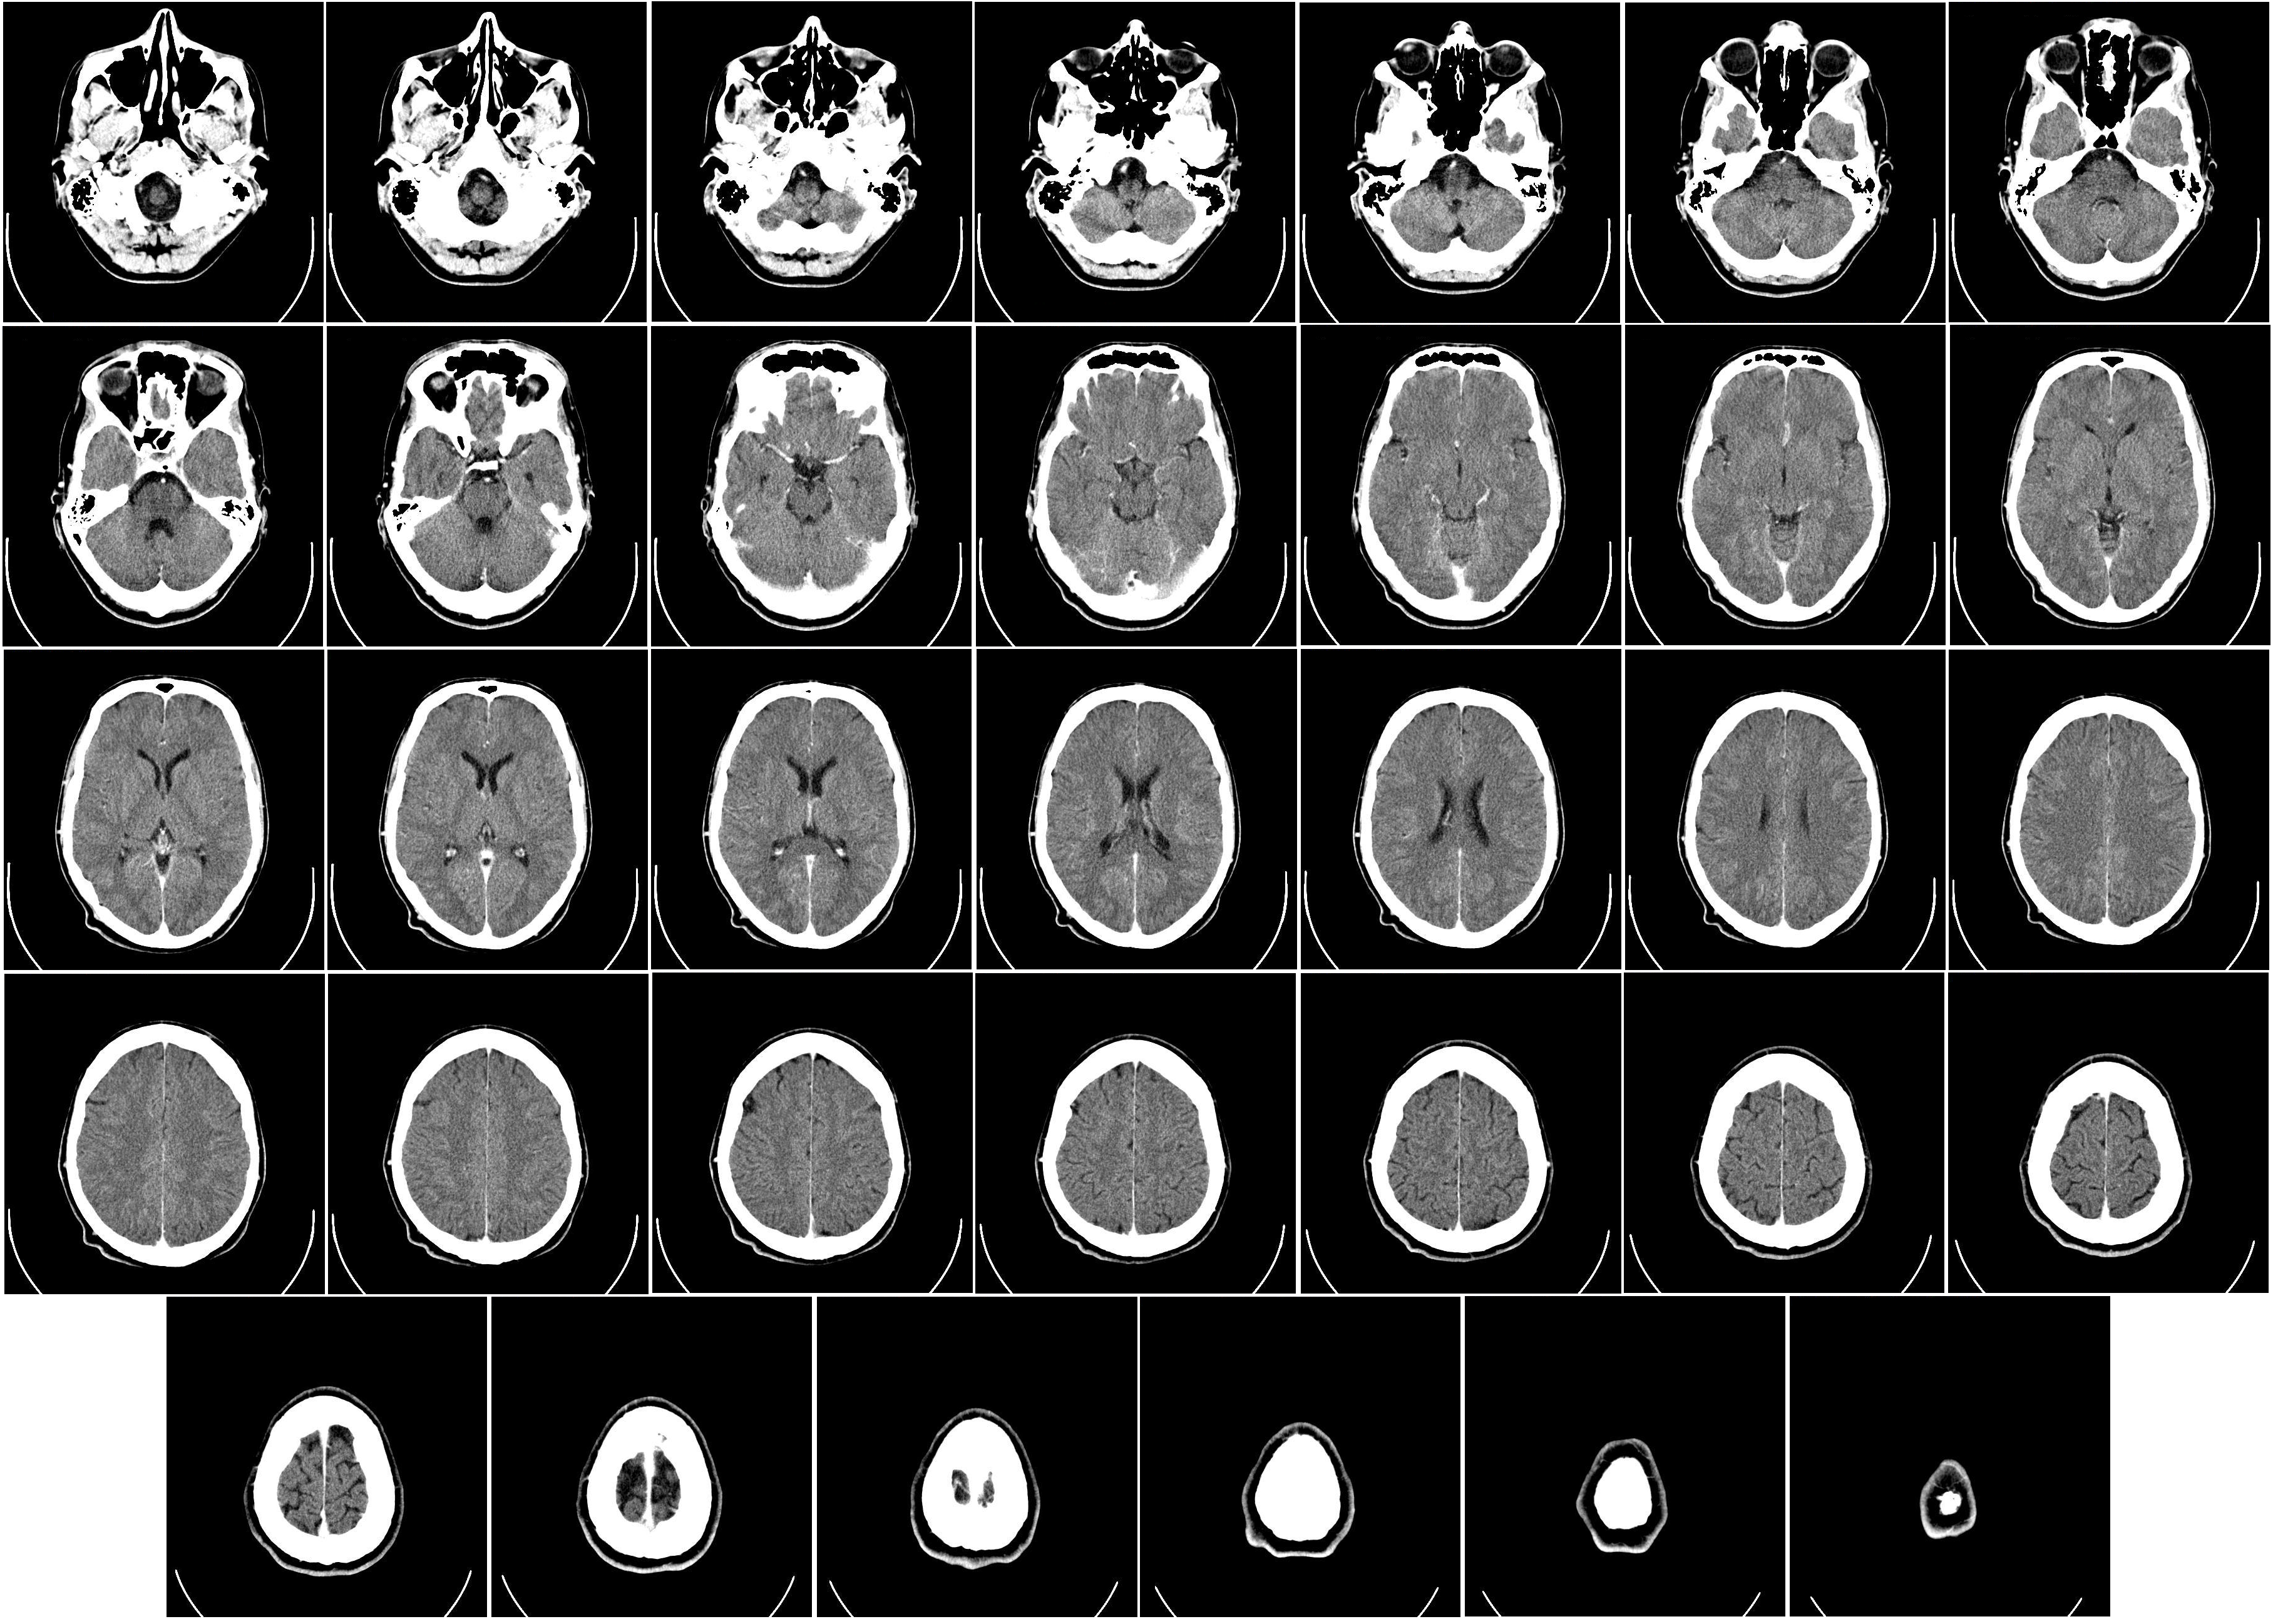
\includegraphics[width=.6\textwidth]{images/ct}
	\end{center}
\end{frame}

\begin{frame}
	\frametitle{1987: 3D}
	\begin{itemize}
		\item Marching Cubes/Isosurfaces (CT)
	\end{itemize}
	\begin{center}
		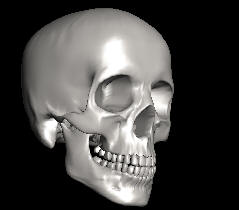
\includegraphics[width=.4\textwidth,height=.4\textheight]{images/marching}
	\end{center}
\end{frame}

\begin{frame}
	\frametitle{More dimensions}
	Higher dimensional data due to:
	\begin{itemize}
		\item Time-variance
		\item Multi-field (DTI, tensors)
		\item Simulation
		\item Multiple sources
			\begin{itemize}
				\item Multi-subject
				\item Multi-modal
			\end{itemize}
	\end{itemize}
\end{frame}

\begin{frame}
	\frametitle{More dimensions}
	\textbf{Solutions:}\\
	Add interactivity:
	\begin{itemize}
		\item Multi-touch devices allow for more flexibility
	\end{itemize}
	Improved visualizations:\\
	\begin{itemize}
		\item Topological methods
		\item Illustrative visualizations
	\end{itemize}
	versus
	\begin{itemize}
		\item Hyper-realism
	\end{itemize}
\end{frame}

\begin{frame}
	\frametitle{2001: 4D}
	\begin{itemize}
		\item Tory et al. (2001) use isosurfaces to visualise MS lesions over
			\textbf{time} (MRI)
	\end{itemize}
	\begin{center}
		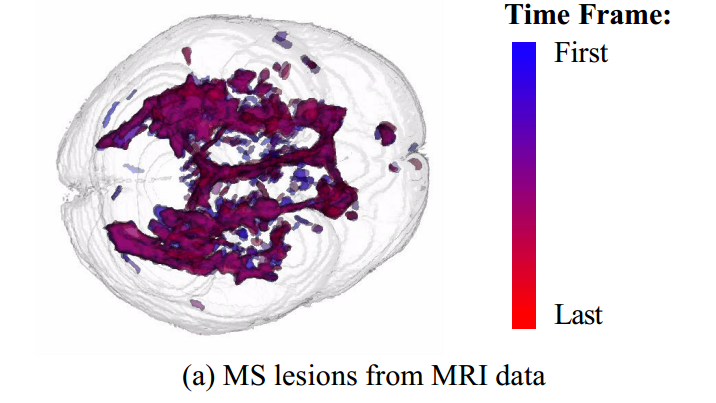
\includegraphics[width=.8\textwidth]{images/ms_time}
	\end{center}
\end{frame}

\begin{frame}
	\frametitle{Mappings:}
	\begin{itemize}
		\item standardized mapping of higher dimensions to lower dimension
		\item greatly facilitates interpretation of data
		\item enables study with minimum interaction
	\end{itemize}
	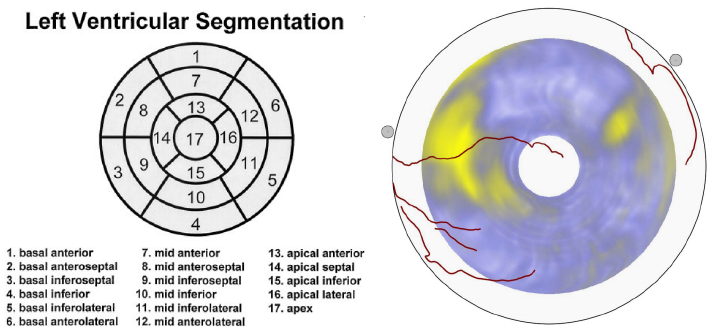
\includegraphics[width=\textwidth]{images/heart}
\end{frame}

\begin{frame}
	\frametitle{Illustrative:} %(Zachow et al. 2009):
	\begin{itemize}
		\item create renditions that consider perceptual abilities of humans
		\item non-photorealistic rendering
		\item for example: boundary enhancement, transfer-functions based on
gradients
	\end{itemize}
	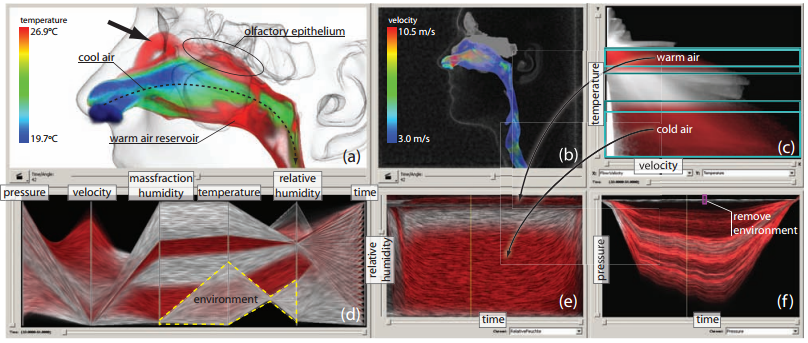
\includegraphics[width=\textwidth]{images/nose}
\end{frame}

\begin{frame}
	\frametitle{Illustrative:} % - colon unfolding (Tietjen et al. 2005):
	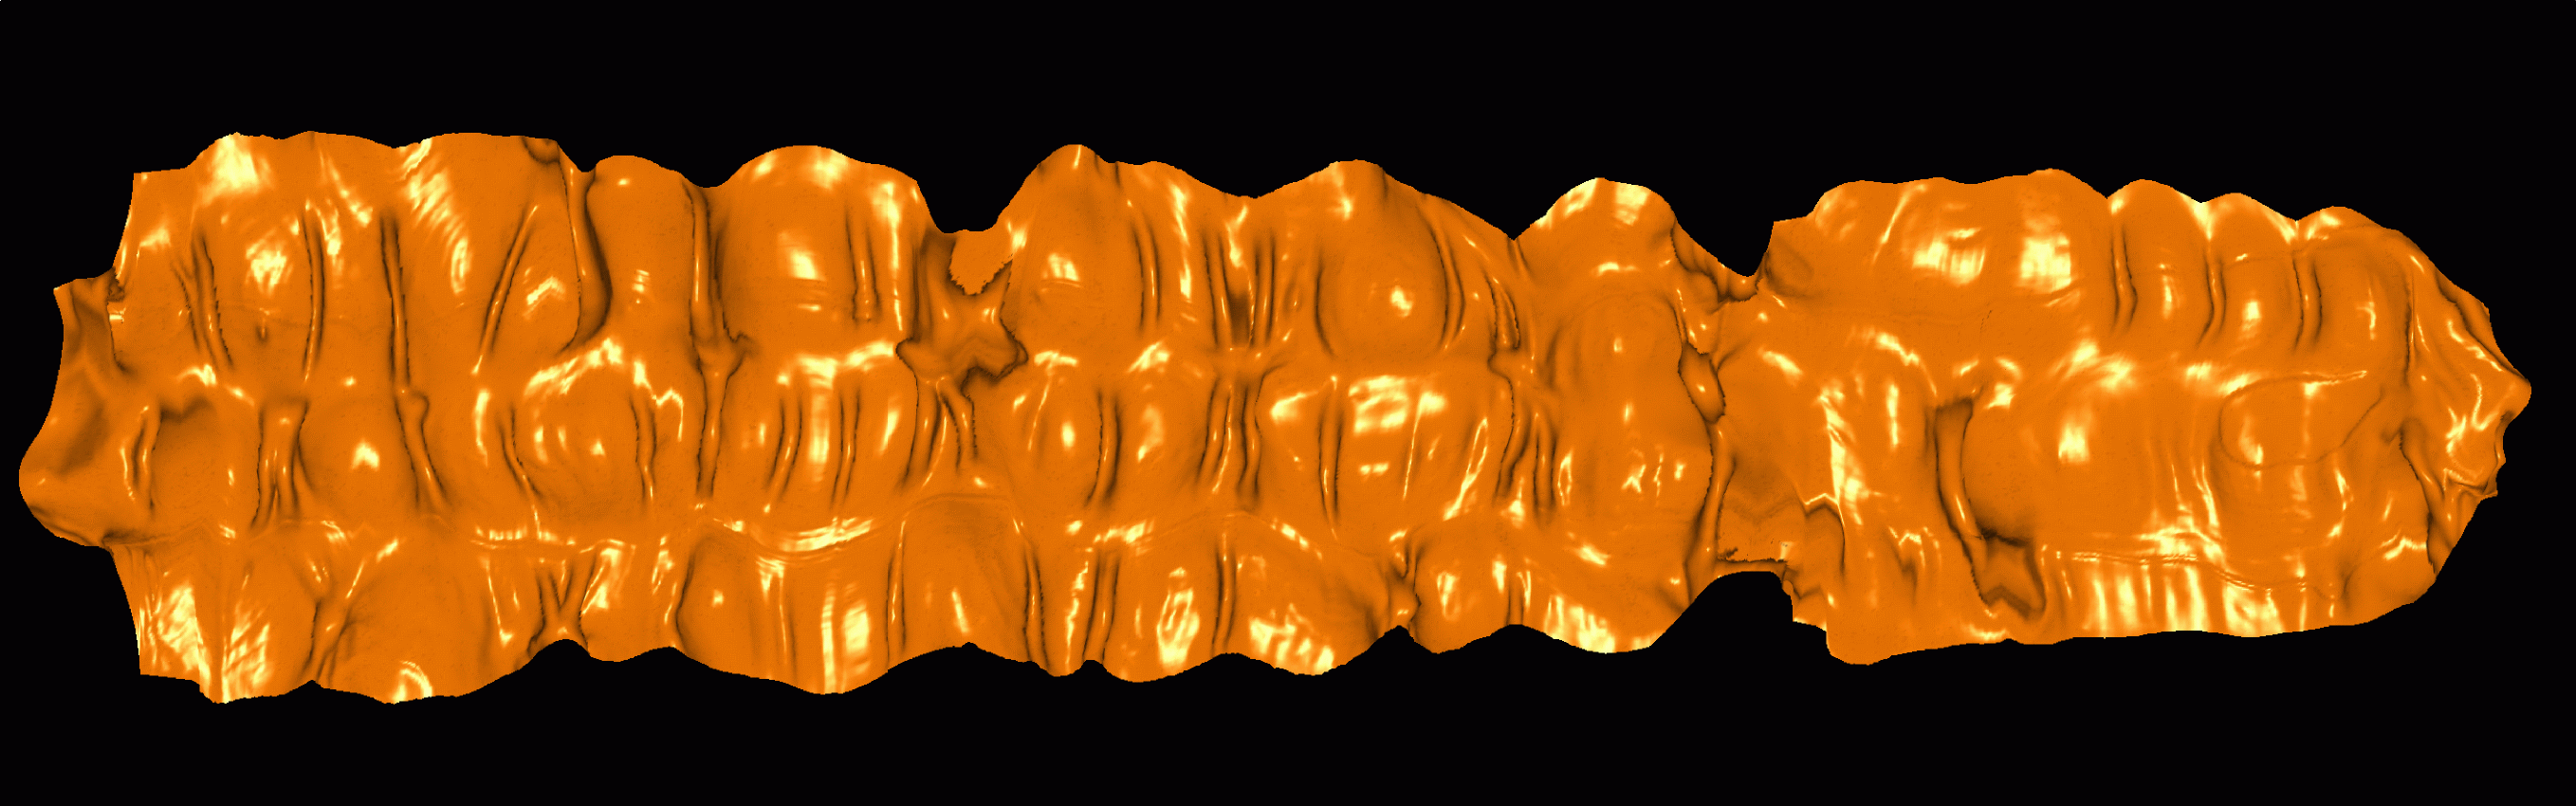
\includegraphics[width=\textwidth]{images/colon}
\end{frame}

\begin{frame}
	\frametitle{DTI:} % 2.3
	Diffusion Tensor Imaging, an MRI-based acquisition modality
	\begin{itemize}
		\item able to capture presence and orientation of fibrous structures
(e.g. muscles)
		\item first examples of natively multi-field medical data %(multiple parameters over
the same spatio temporal domain)
	\end{itemize}
\end{frame}

\begin{frame}
	\frametitle{DTI:}
	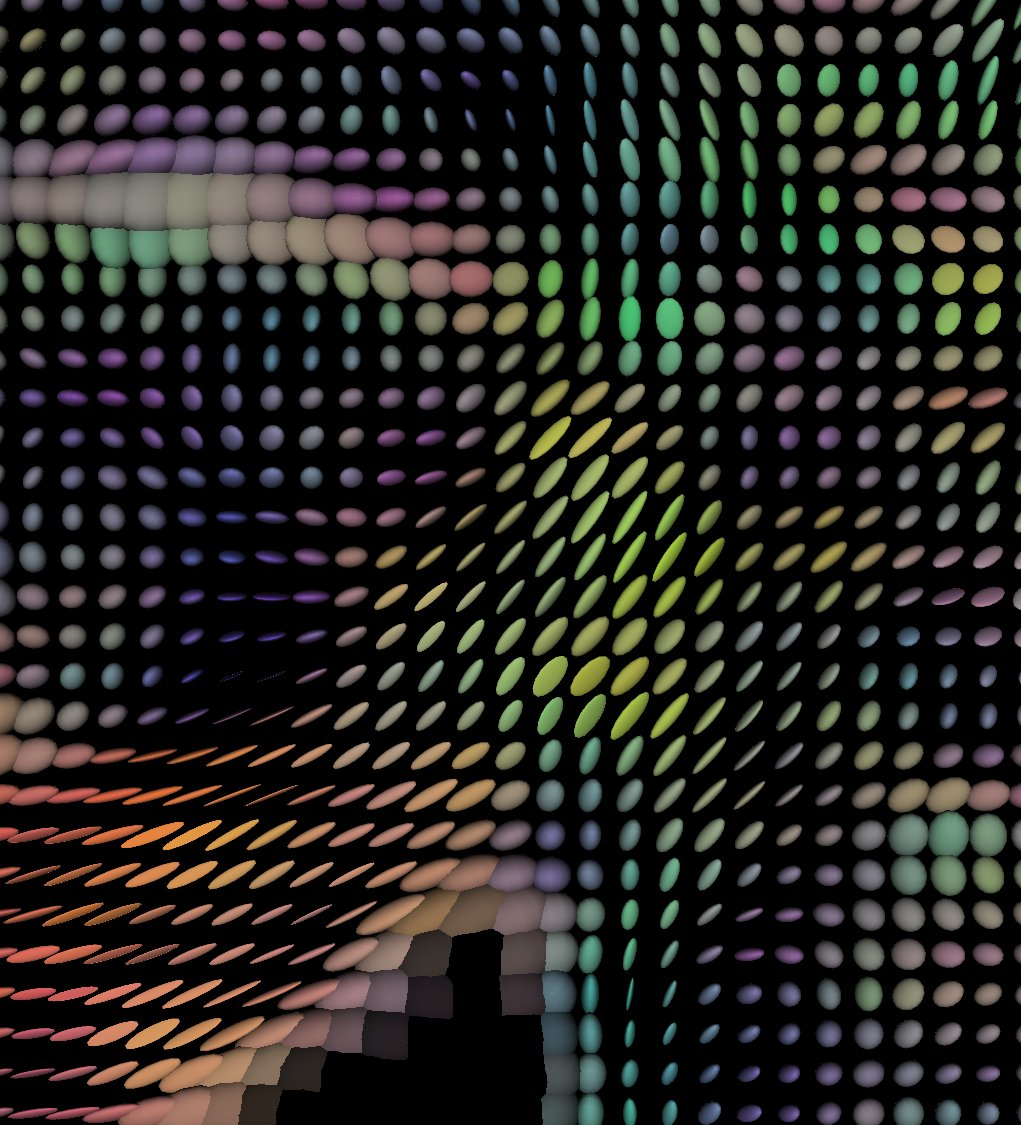
\includegraphics[width=\textwidth]{images/dti}
\end{frame}

\begin{frame}
	\frametitle{DTI:}
	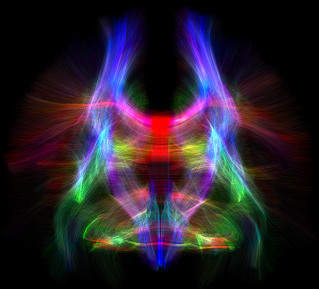
\includegraphics[width=\textwidth]{images/tractography}
\end{frame}

\begin{frame}
	%\frametitle{With great computing power comes great medical visualization}
	\frametitle{Realism:}
	\begin{itemize}
		\item photo-realism
		\item hyper-realism (visual art)
		\item additional realistic details convey info better?
		\item should be explored!
	\end{itemize}
\end{frame}

\begin{frame}
	\frametitle{Realism:}
	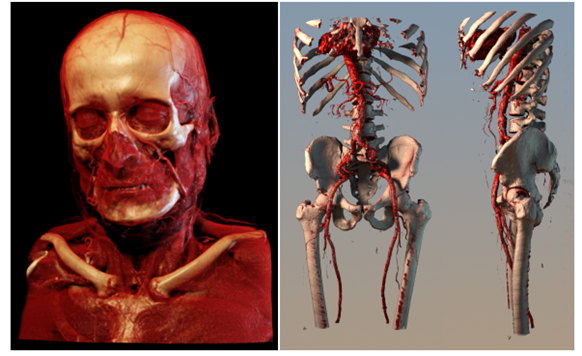
\includegraphics[width=\textwidth]{images/medical_visualisation}
\end{frame}

\begin{frame}
	\frametitle{Realism:}
	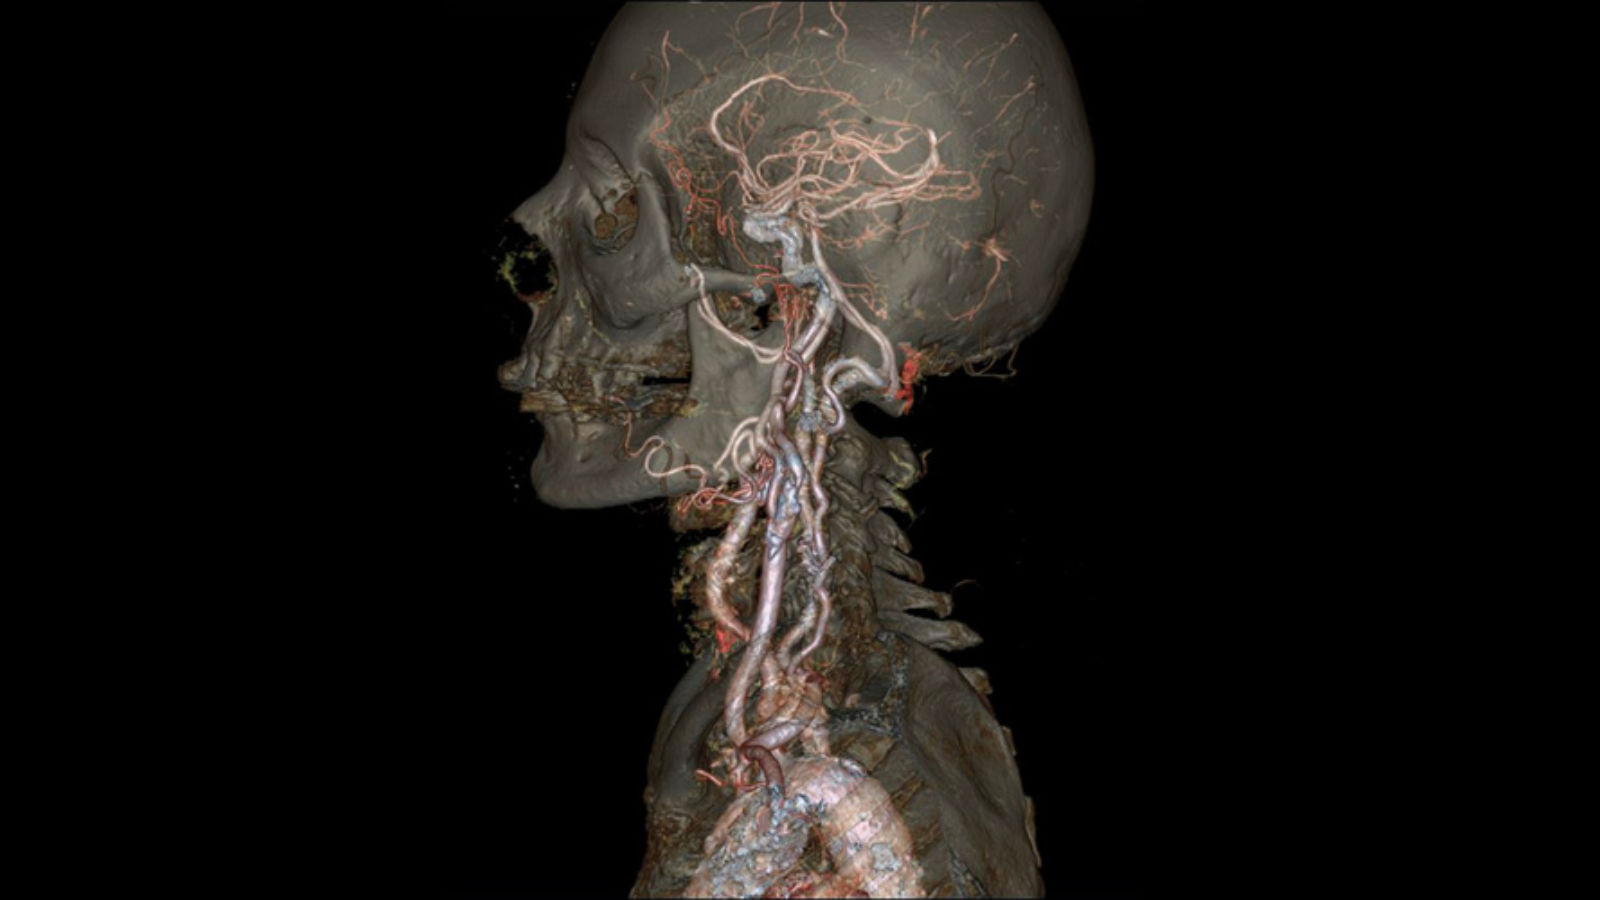
\includegraphics[width=\textwidth]{images/realistic_transparent}
\end{frame}

\begin{frame}
	\frametitle{Conclusions:}
	\begin{itemize}
		\item identified problems for the next decade
	\end{itemize}
\end{frame}


\end{document}
% vim: spell
